\documentclass[9pt,twocolumn,twoside]{../../styles/osajnl}
\usepackage{fancyvrb}
\journal{i524} 

\title{Hive}

\author[1,*, +]{Diksha Yadav}

\affil[1]{School of Informatics and Computing, Bloomington, IN 47408, U.S.A.}

\affil[*]{Corresponding authors: yadavd@umail.iu.edu}

\affil[+]{HID - S17-IR-2044}

\dates{Paper-002, \today}

\ociscodes{Hive, Hadoop, HiveQL, SQL}

% replace this with your url in github/gitlab
\doi{\url{https://github.com/diksha2112/sp17-i524/tree/master/paper2/S17-IR-2044/report.pdf}}


\begin{abstract}
Hive is an open source data warehousing solution which is built on top of Hadoop. It structures data into understandable and conventional database terms like tables, columns, rows and partitions. It supports HiveQL queries which have structure like SQL queries. HiveQL queries are compiled to map reduce jobs which are then executed by Hadoop. Hive also contains Metastore which includes schemas and statistics which is useful in query compilation, optimization and data exploration.

\end{abstract}

\setboolean{displaycopyright}{true}

\begin{document}

\maketitle

\TODO{This review document is provided for you to achieve your
  best. We have listed a number of obvious opportunities for
  improvement. When improving it, please keep this copy untouched and
  instead focus on improving report.tex. The review does not include
  all possible improvement suggestions and for each comment you may
  want to check if it applies elsewhere in the document.}

\TODO{Please include the correct link to your report on the
  \emph{cloudmesh} user's Github account, not \emph{diksha2112}'s.}

\TODO{Your paper does not meet the length requirements for the
  assignment. Moreover, what you have included is more like a random
  selection of tidbits about Hive than a coherent paper. You need to
  rewrite the paper.}

\TODO{Assessment: Major revisions required.}

\section{Introduction}
The reason behind development of Hive is making it easier for end users to use Hadoop. Map reduce \TODO{MapReduce} programs were required to be developed by users for simple to complex tasks. It lacked expressiveness like query language. \TODO{Not the case. MapReduce has more expresiveness than Hive, that is, you can express more programs with MapReduce than with Hive. Hive simply makes common use cases of MapReduce easier to write in a familiar, SQL-like environment.} So, it was a time consuming and difficult task for end users to use Hadoop. For solving this problem Hive was built in January 2007 and open sourced in August 2008.
Hive is an open source data warehousing solution which is built on top of Hadoop. It structures data into understandable and conventional database terms like tables, columns, rows and partitions. It supports HiveQL queries which have structure like SQL queries. HiveQL queries are compiled to map reduce \TE jobs which are then executed by Hadoop. Hive also contains Metastore which includes schemas and statistics which is useful in query compilation, optimization and data exploration\cite{wk}

\section{Architecture}

\TODO{This section is incomplete. There is very little detail about the different parts of the architecture, there is no motivation for why they exists, or explanation of how they fit togehter. They are not even formatted properly in the text. The architecture figure is not referenced anywhere in the text. Please revisit. }

Hive architecture includes,
Database-It consists of tables created by the user.
Metastore-It contains information about the system. It can be accessed by different components as and when needed.
Interfaces-User interface and Application programming interface both are present in hive.
Driver-manage HiveQL statements at every stage.
Query compiler-It compiles HiveQL queries to acyclic graphs (directed) representing map reduce tasks.
Execution Engine- It executes the tasks generated by the compiler.
Hive Server- It provide JDBC/ODBC server and thrift interface\cite{td}

\begin{figure}[htbp]
	\centering
	\fbox{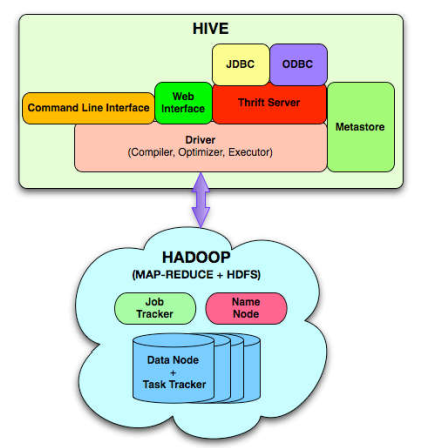
\includegraphics[width=\linewidth]{images/harch.png}}
	\caption{Hive Architecture \TODO{Did you create this figure? If not, you need to provide a reference to where you got it from.}}
	\label{fig:Hive-arch}
\end{figure}

\section{HiveQL Query Format}
SELECT [ALL | DISTINCT] select-expr, select-expr, ...\newline
FROM table-reference\newline
[WHERE where-condition]\newline
[GROUP BY col-list]\newline
[HAVING having-condition]\newline
[CLUSTER BY col-list | [DISTRIBUTE BY col-list] [SORT BY col-list]]\newline
[LIMIT number]\newline
\cite{p1}\newline

\TODO{This is out of scope for the paper. In an overview paper like this you don't need to provide the format for a single SELECT statement. Anyone can look this up in the docs.}

\section{System Requirements}
Hive is cross platform. So, It does not need any specific operating system to work.

\TODO{But what are the system requirements?}

\section{Comparison of Hive with Other Traditional Databases}
Traditional databases follow schema on write approach while Hive follows schema on read approach. In schema on write, databases checks at load time if the data follows the table representation given by user while in schema on read approach, it is checked at run time only. This saves the time for hive to load the data when traditional databases takes longer time\cite{p2}

\TODO{Is this the only or even most important point to compare Hive against other platforms on?}

\section{Popularity of Hive}
The popularity of hive increasing with time. This can be proved by the following plot made by DB Engines Ranking. It ranks database management systems according to their status and popularity.
Following plot shows popularity of hive with time. \TODO{Why is it important that Hive's popularity has increased over time? In addition, this is not the proper way to cite a source.}

\begin{figure}[htbp]
	\centering
	\fbox{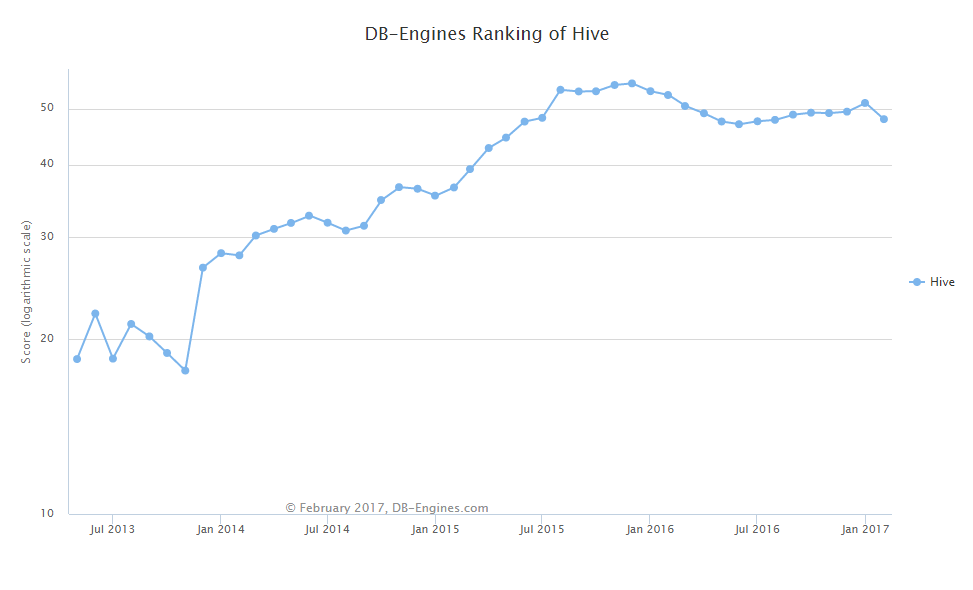
\includegraphics[width=\linewidth]{images/hgraph.png}}
	\caption{Hive Popularity}
	\label{fig:HivePopularity}
\end{figure}
\cite{rank}

\section{Resources for learning Hive}
Someone new to hive can start learning it by going through the following links in sequence:
Install Hive\url{https://www.edureka.co/blog/apache-hive-installation-on-ubuntu?utm_source=quora&utm_medium=crosspost&utm_campaign=social-media-edureka-ab}\newline
Hive Tutorial\url{https://www.edureka.co/blog/hive-tutorial/?utm_source=quora&utm_medium=crosspost&utm_campaign=social-media-edureka-ab}\newline
Top Hive commands with examples\url{https://www.edureka.co/blog/hive-commands-with-examples?utm_source=quora&utm_medium=crosspost&utm_campaign=social-media-edureka-ab}\newline

\section{Acknowledgement}
I am also grateful to Dr. Gregor von Laszewski for providing the appropriate paper template.


\section{Conclusion}
Since Hive is making the use of Hadoop easier for users, its popularity is increasing with time.
\TODO{The conclusion needs to summarize the paper. I don't know what to make of this sentence about Hive's popularity.}

% Bibliography

\bibliography{references}

\end{document}
